\chapter{Optical Enhancement of Core-Shell Nanowire} \label{data}

Given that the profound enhancement of optoeletronic properties of nanowires is
the major theme of this dissertation, it is dutiful to first summarize the
major experimental results, such as fabrication techniques and characteristics of
core-shell nanowires (CSNWs).

A CSNW is a quasi-one dimensional structure with a wide band gap materials,
such as AlGaAs, wrapping around a low band gap semiconductor, such as GaAs. It
is expected that the lower dimensionality of electronic states in CSNW to have
a significant influence on both optical and electrical properties of the
structure. For instantce, electron systems in lower dimensions are adequately
treated through perturbation methods, and the correlations among electrons are
much more significant due to higher degrees of confinement. The electrons can
be moving in the direction of NW growth axis and any small or localized
interaction can cause a collective response from the whole system. Importantly,
this one-dimensional electron system (1DES) can experimentally be realized in
various material systems. These include carbon nanotubes, electrons at the
edges of a two-dimensional electron system (2DES), and in NWs.

Electrically it is important account for the electron correlations in order to
determine the behavior of the structure. The significant values of exchange and
correlation energies in 1DES, makes them an interesting candidate for probing
their energy dynamics, and especially the interaction with light. This,
however, imposes various experimental challenges and theoretical considerations
and will be discussed in the following sections.

\section{Growth of Nanowires}

Freestanding quasi-one-dimensional semiconductor NWs based on III-V compound
semiconductors, owing to their unique physical
properties~\cite{huang2002gallium,Law:2004gl}, are considered ideal building
blocks for the realization of photonic and electronic nano-scale devices.

Currently, two bottom-up approaches to the fabrication of freestanding
nanowires are considered: (i) selective area epitaxy
(SAE)~\cite{motohisa2004catalyst} and (ii) metal-catalyst assisted growth
through the so-called vapor-liquid-solid (VLS) mechanism~\cite{wagner1964vapor,
givargizov1975fundamental}. The latter method relies on the alloying of a metal
catalyst (usually Au) nanoparticle with the semiconductor constituent elements,
supplied through a vapor phase. The as-formed alloy acts as an initial
nucleation site for the material and further guides the nanowire growth, the
diameter of the nanowire being controlled by that of the metal
nanoparticle~\cite{cui2001diameter}.

An advantage of the VLS method over SAE is that it does not require
nanolithography processing of the substrate; furthermore, it is compatible with
most advanced epitaxial growth techniques for III-V compounds, such as
molecular beam epitaxy (MBE)~\cite{Zhou:2009cg,colombo2008ga}, chemical beam
epitaxy (CBE)~\cite{ercolani2009inas}, and metalorganic vapor phase epitaxy
(MOVPE)~\cite{Noborisaka:2005hh,paiano2006size}. In addition, the growth of
expitaxial NWs allows precise control over the material composition and/or
intentional doping along the NW length (i.e., growth direction). Most commonly
used precursors of group-V elements are arsine ($AsH_3$) and phosphine,
however, instead of using the toxic hydrides, the alkyl-substituted arsine and
phosphine molecules will be much more safer and improve the materials'
electronic properties. The detailed fabrication techniques will be discussed
next.

GaAs nanowires were grown by low (50mbar) pressure MOVPE using an Aixtron
reactor model AIX200 RD. Trimethylgallium (TMGa) and tertiarybutylarsine (TBAs)
were used as gallium and arsenic precursors, respectively. Au nanoparticle
deposited on $(\bar{1}\bar{1}\bar{1})B$ GaAs were used to catalyze the nanowire
growth. To this purpose, VGF-grown semi-insulating (undoped) GaAs wafers
oriented $(\bar{1}\bar{1}\bar{1})B$ were used. The substrates were then first
degreased in isopropanol vapors, etched in $4H_2SO_4:1H_2O_2:2H_2O$ solution
for 8 min at around $40\,^{\circ}\mathrm{c}$, rinsed in de-ionized water and
finally dried under pure $N_2$. Au nanoparticles with $\sim 60 nm$ diameters
were prepared by reaction of $HAuCl_4$ with sodium citrate in aqueous solution
and randomly deposited on the as-prepared GaAs surface by dropping a small
amount of colloidal solution onto the substrate. The solvent (water) was then
evaporated by holding the samples on a hot plate (in air) or a few minutes; Au
nanoparticle surface densities thus achieved ranged around
$(1-4)\times{10}^8{cm}^{-2}$.

After loading the sample into the reactor chamber, its temperature was raised,
and sample annealing was then performed for 10 min to absorb GaAs surface
oxides and organic residues originating from the Au nanoparticle synthesis.
This annealing step would also allow the initial uptake of Ga atoms from the
GaAs substrate into the Au nanoparticles. After ramping down the sample
temperature to the final growth value, TMGa was admitted to the reactor chamber
and the growth was initiated.

\section{Scanning Electron Microscopy Images} 

The nanowire morphology and dimensions were studied by scanning electron
microscopy (SEM) observations using a Dual Beam Scanning Electron/Focused Ion
Beam Microscope model FEI Helios; a primary electron beam acceleration voltage
of 15 kV and a working distance of 10 mm were employed. Figure~\ref{SEMNW} is
top view scanning electron microscopy (SEM) image of nanowires with $\sim100nm$
diameter core of GaAs, $\sim40nm$ thick of AlGaAs shell, and an additional
$\sim5nm$ GaAs cap layer. The four figures show the CSNWs array at different
magnifications and view angles. These images demonstrate the rather sparse
distribution of the wires. In addition, the wires are not fully arrayed with
various growth directions and lengths. The most magnified view for the left
bottom figure clearly indicate the CSNWs have hexagonal structure and tapering
effect along the wire growth direction.

\begin{figure}
  \caption{Scanning Electron Microscopy image of as-grown GaAs/AlGaAs core-shell nanowires on Si taken at different magnifications and view angles (Image courtesy of Dr.Pouya Dianat)}
  \centering
  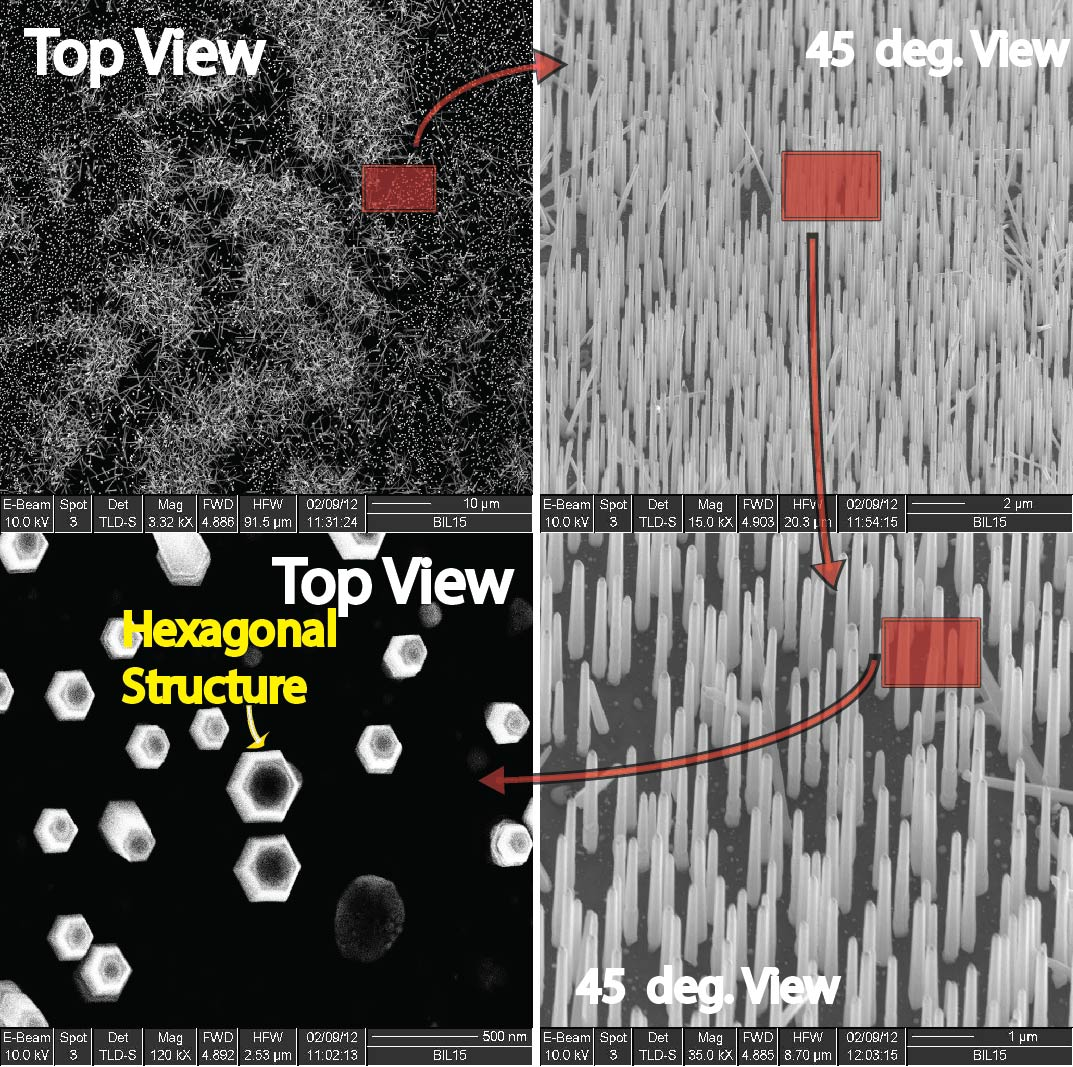
\includegraphics[width=\textwidth]{pictures/Data/SEMNW}
  \label{SEMNW}
\end{figure}

\section{Electrical Characterization of Nanowire}

The as-grown CSNWs are used to perform optical characterization measurement.
However, in order to measure the CSNWs electrical performance, additional
treatments have been taken to make Ohmic contacts between nanowires and
transmission lines. Figure~\ref{ContactNW} show the SEM image of one dispersed
core-shell nanowire connecting with the transmission line by Focus Ion Beam
(FIB) for (left) I-V and (right) C-V measurement. The CSNWs were first detached
from the as-grown Si or GaAs substrate by
ultrasonication~\cite{wang2007direct,wan2004fabrication} in an ethanol bath and
dispersed between two transmission lines, then contacted with the transmission
lines by FIB using platinum metal.

Characteristic current-voltage (I-V) curves of the nanowire device are given in
Fig.~\ref{CSNWIVlight}. The I-V curve exhibits rectifying behavior, confirming
that the device is a well=behaved diode structure with the electric contact on
one side (Al) ohmic and the other (Pt) Schottky. The reverse bias dark current
of the device is very small, $\sim20pA$ at -1V, and could be further improved
by properly passivating the CSNW surface. Upon illumination, the device shows a
prnounced photovoltaic response due to the built-in potential from the Schottky
junction. The short length of the nanowire device and the large depleted region
by the built-in potential enable the nanowire photodetector to be operated at
zero bias. Fig.~\ref{CSNWIVlight} shows the photocurrent of the device at zero
bias as a function of irradiance. The linearity of the device was demonstrated
up to at least at a 632 nm wavelength. The excellent linear response is in part
based on the good crystalline quality of the nanowires, as confirmed by
transmission electron microscopy. In addition, the capactiance of a typical
device () is calculated to be 5 aF based on a simple parallel-plate model and
thus its cutoff frequency is mainly limited by the transit time of the
photo-generated charge carriers in the device, which may in principle reach ~
100 GHz after certain parameter opti 

\begin{figure}
  \caption{Scanning Electron Microscopy (SEM) image of one dispersed core-shell nanowire connecting with the transmission line by Focus Ion Beam (FIB). (left) NW with small contact pad to connect the transmission line for I-V measurement. (right) NW with large contact pad to connect the transmission line for C-V measurement.}
  \centering
  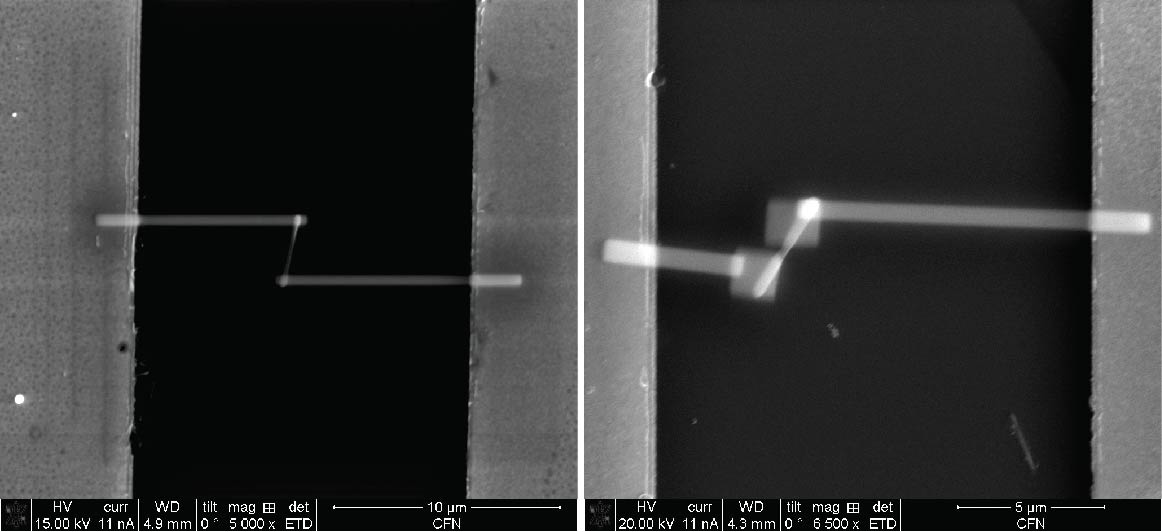
\includegraphics[width=\textwidth]{pictures/Data/ContactNW}
  \label{ContactNW}
\end{figure}

\begin{figure}
  \caption{Current versus Voltage Measurement under illumination of Single Core-Shell Nanowire.}
  \centering
  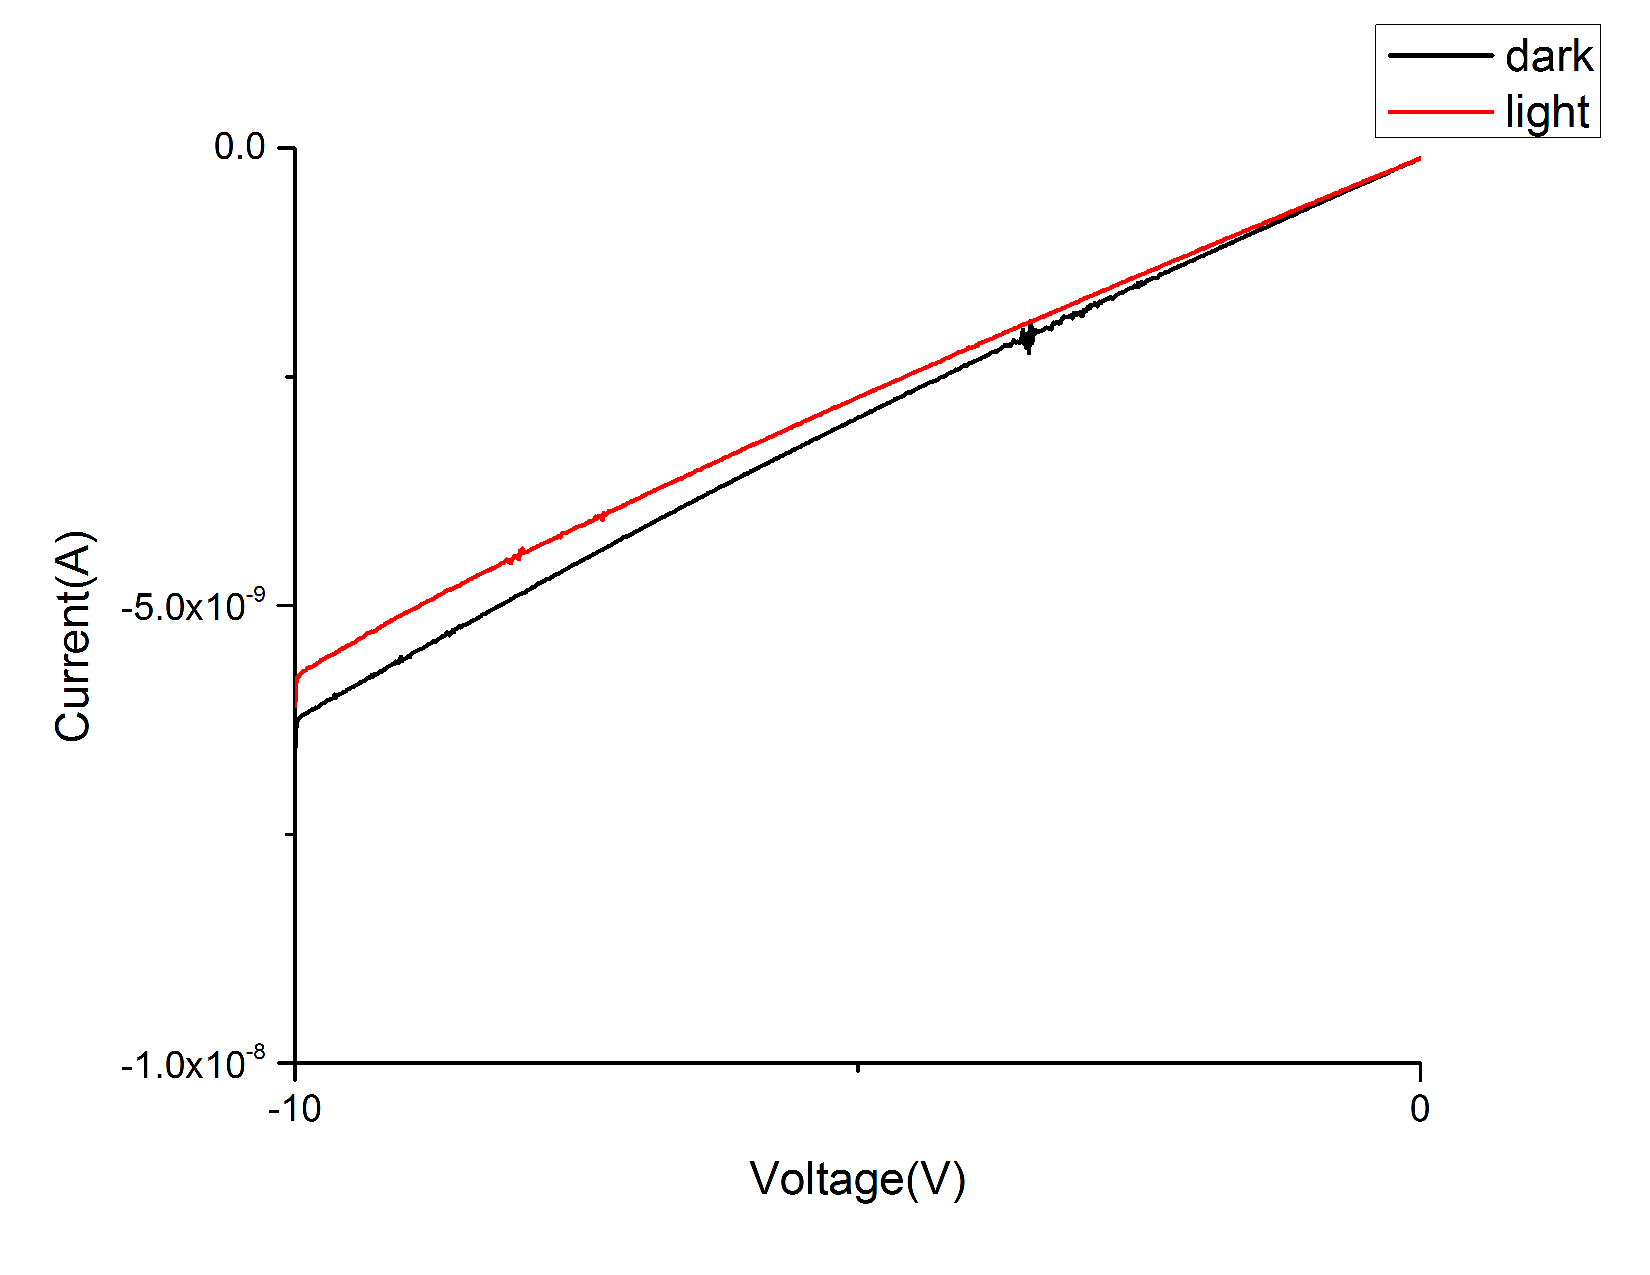
\includegraphics[width=\textwidth]{pictures/Data/CSNWIVlight}
  \label{CSNWIVlight}
\end{figure}

\begin{figure}
  \caption{Capacitance versus Voltage Measurement under illumination of Single Core-Shell Nanowire.}
  \centering
  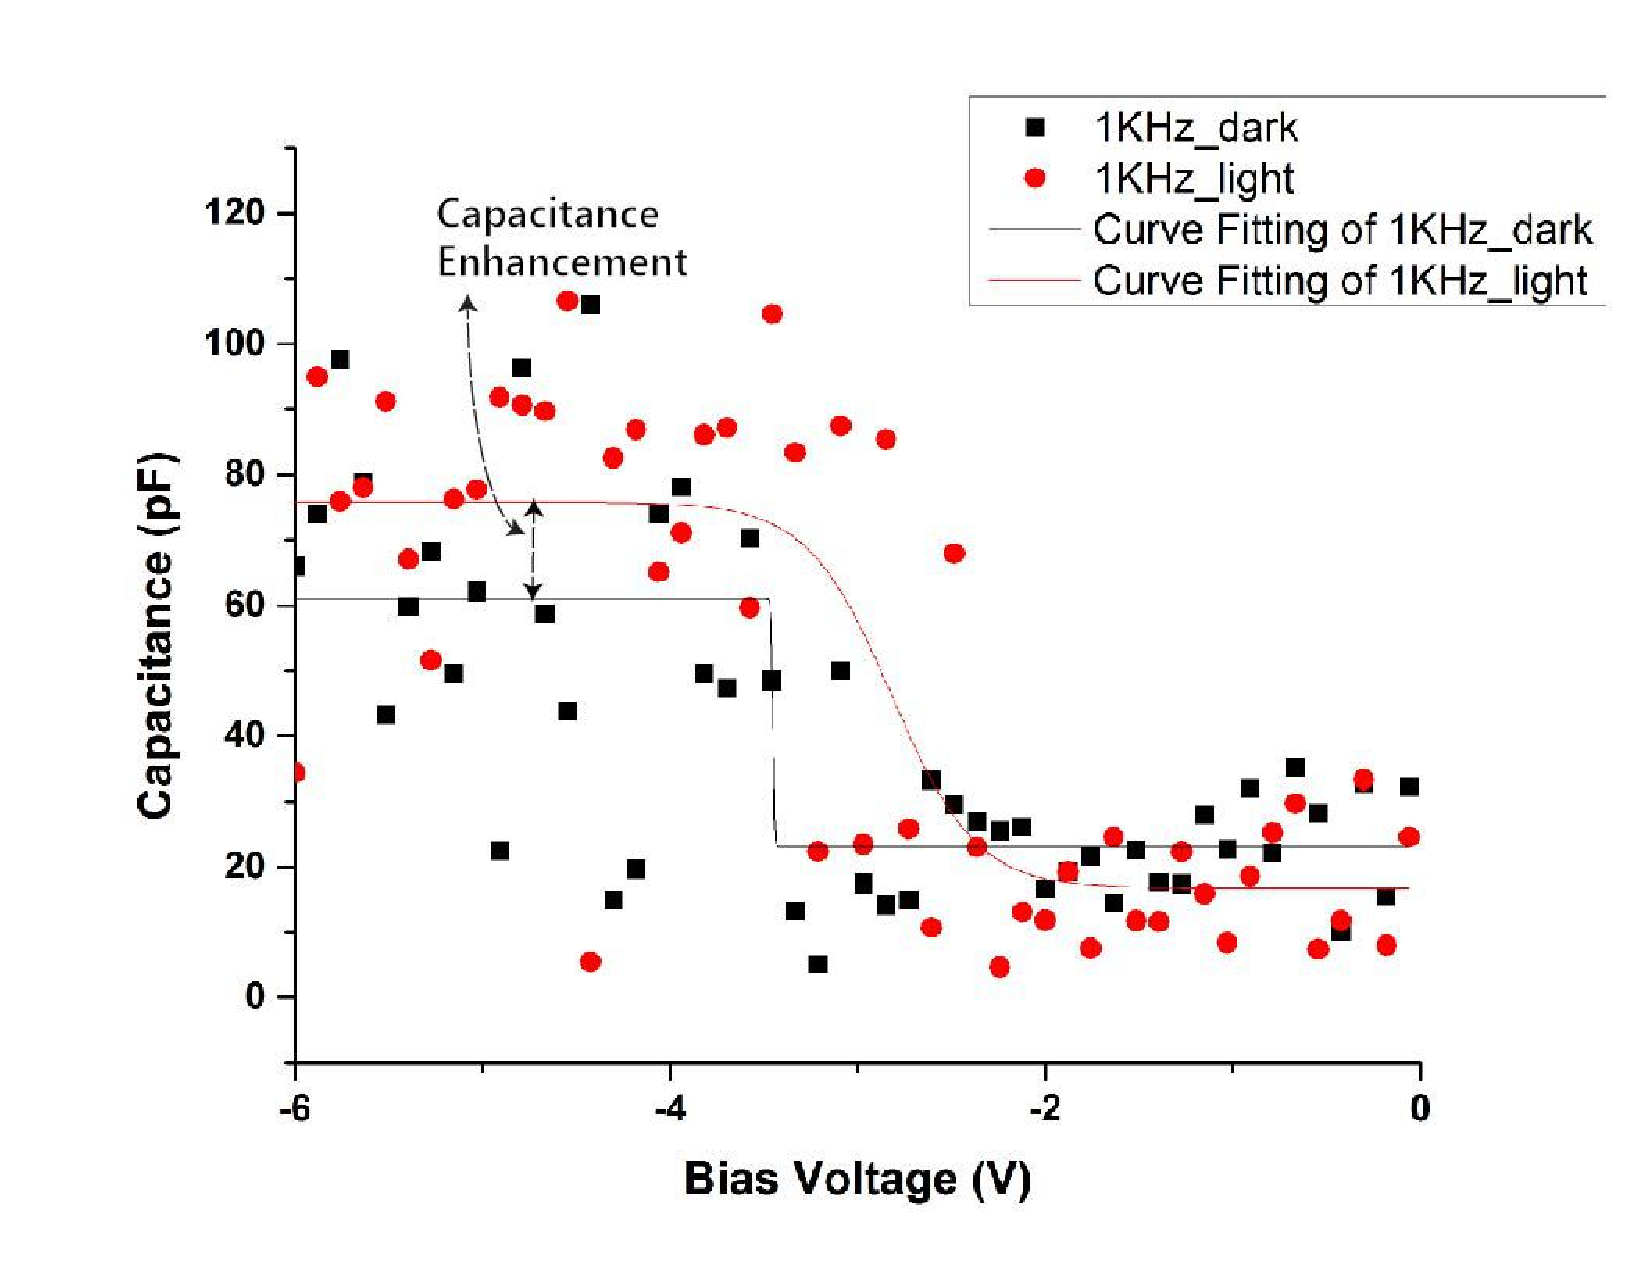
\includegraphics[width=\textwidth]{pictures/Data/CSNWCVlight}
  \label{CSNWCVlight}
\end{figure}

\section{Electro-Optically Sampled Time Response}

The electro-optic sampling (EOS) set up is shown in Fig~\ref{NWEOS} (a). In
essence, the EOS is an ultrafast sampling oscilloscope that uses femtosecond
laser pulses to excite optoelectronic transients and then measures the
electronic response by probing the refractive index change of an electro-optic
crystal placed on top of the device and/or transmission line. In our setup, the
laser is split into two paths: one path, the pump beam, is coupled into a fiber
to excite the device and the other path, probe beam, passes through a
LiTaO\textsubscript{3} crystal to sample the electric field of the propagating
response. As shown in Fig.~\ref{NWEOS} (a, b) the CSNW were placed in the
middle of a coplanar transmission line (TL), and connected to the TL by Focused
Ion Beam (FIB) lithography. The distance between the two FIB contacts is
\textasciitilde{}3.5 $\mu{m}$.

By varying the optical path of the sampling beam, the temporal response of the
device is observed with a time resolution limited by the laser pulse width and
the response of the electro-optic crystal. The amplitude sensitivity is limited
by the noise in our detection system. We modulated the switching beam at 80 kHz
and performed phase-sensitive detection with a lock-in amplifier on the light
analyzed (with a polarizer and differential detection) from the
LiTaO\textsubscript{3} crystal, in order to increase the sensitivity to sub-mV
levels. In this experiment, \textasciitilde{}100 fs pulses from a Ti:sapphire
laser with a center wavelength of 830 nm were split into the two paths. The
path that is coupled into a fiber to excite the device under test (DUT) is
dispersed by the fiber and excites as a 400 fs chirped optical pulse.  The
second laser path that passes through the LiTaO\textsubscript{3} crystal to
sample the propagating electric field broadens slightly to a 150 fs optical
pulse at the crystal. The photodetectors' electronic response is coupled to a
coplanar strip (CPS) transmission line. The separation from the fiber exciting
the device to the optical sampling crystal is 250 μm. The CPS transmission line
is contacted with microwave probes for dc bias and \textless{} 50 GHz
measurements. Bias values from -10 to +10 V were applied to the CSNW structure
with average optical powers ranging from 250 nW to 10 mW.

The current -- voltage (I-V) measurements in ambient room light (dark)
and under continuous wave (CW) illumination by an 830 nm Ti:sapphire
laser are performed. The CSNW has very low dark current
(\textless{}0.1pA) which increases to 170nA average photocurrent with
2.6 mW of optical power; remarkable for a single wire. This corresponds
to a responsivity of 0.03 A/W, while the responsivity for the same
volume of GaAs in bulk is 0.02x10\textsuperscript{-3} A/W. A three
orders of magnitude increase in the responsivity demonstrates that CSNW
is not only a good absorber but also converts energy more efficiently
compared to their thin film counterparts. This I-V response result shows
that the device is an efficient optical detector mostly due to the
collection of carriers generated outside of the active region, which are
efficiently collected in the low-dimensional electron gas reservoir
which will be discussed shortly.

The time response data for the CSNW is shown in Fig.~\ref{NWEOS} (c) under
applied bias of ±10 V, showing as-measured full-width half-max (FWHM) of
\textasciitilde{}13 ps. Several factors are involved in the temporal response
measured via electro-optic sampling. The overall response comprises three major
elements: 1) the device response, 2) the signal propagation, and 3) the
electro-optic sampling system measurement. The measurement is a combination of
these responses, resulting in a measured signal that is distorted. Thus, the
device's intrinsic speed is even faster when the test set up limitations are
considered.

Given the length of the wire, this result shows higher speed of both electron
and hole transport in the wire. This is due to the electron charge distribution
in the core-shell nanowire. Different from the core-only nanowires or bulk
semiconductor devices, the CSNWs are able to confine electrons primarily at the
hetero-interface of GaAs core and AlGaAs shell, with small amount of electrons
in the core. The movement of these charged carriers are confined in
two-dimensions, forming a two-dimensional electron gas (2DEG) at the
heterojunction. If the CSNW has hexagonal facet more optical excitation
produces more electron-hole pairs, and higher order confinement or
one-dimensional electron gas (1DEG) will be found as six (6) pillars of charge
at the corners of the hexagonal CSNW~\cite{Wang:2015hz}. In addition to the
confined charge carriers' distribution in CSNWs, there is an electric field due
to applied bias that moves the optically generated electrons to the 2DEG/1DEG.
These optically generated carriers perturb the charge reservoirs, eliciting a
collective response that is not limited by the transit of the charges to the
contacts. Analogous to a drop exciting a wave in a reservoir that is detected
more rapidly than the drop's transport by current flow, charge plasma confined
in a semiconductor can transfer energy, hence respond much faster than the
electric field-induced carrier drift current.

\begin{figure}
  \caption{(a) Electro-optic sampling (EOS) time response measurement set up: RF probe is at one end of a transmission line in the middle of which the NW is contacted and is excited by 400 fs pulses of light delivered by fiber; probe beam samples the electric field through the electro-optic crystal. (b) Image of the FIB-contacted NWs. (c) Time response data.}
  \centering
  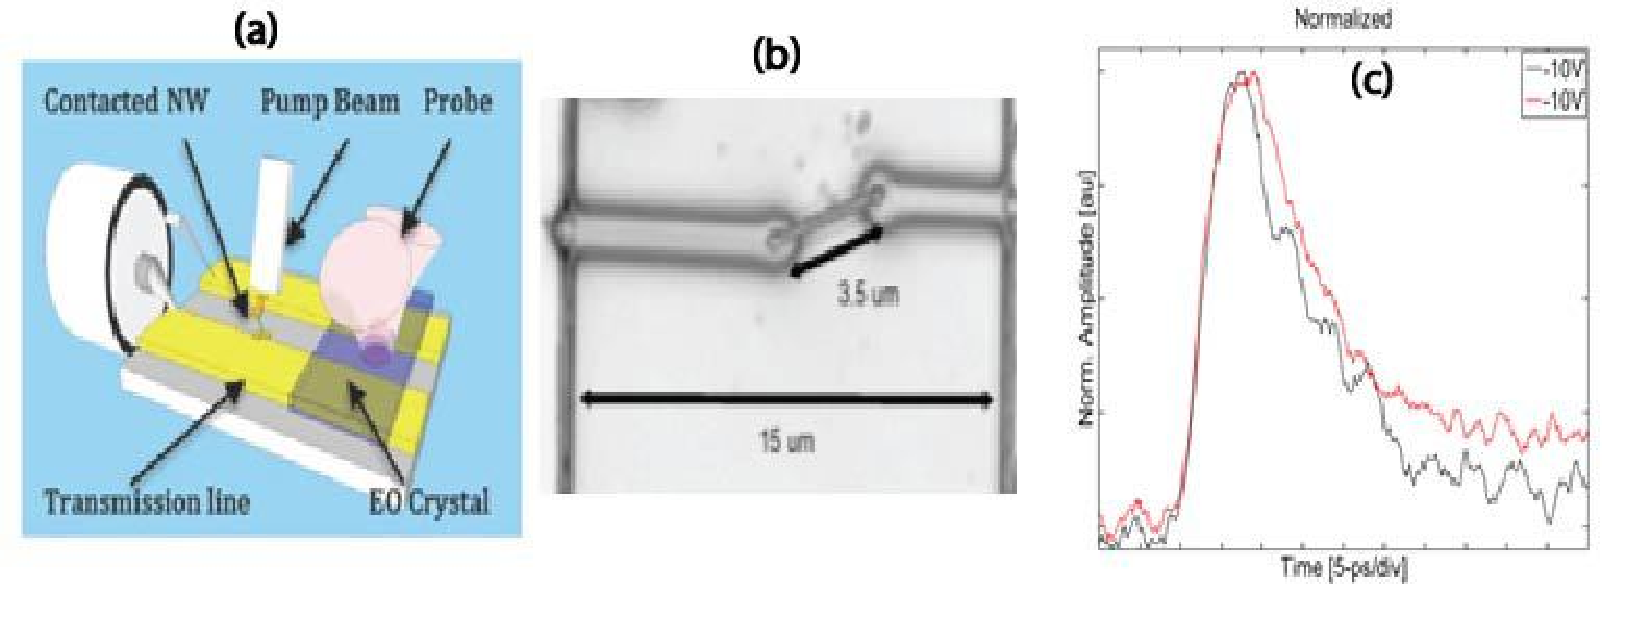
\includegraphics[width=\textwidth]{pictures/Data/NWEOS}
  \label{NWEOS}
\end{figure}

In conclusion, we use an electro-optically sampling measurement technique to
demonstrate a high-responsivity and high-speed opto-electronic device which may
be constructed based on the collective response of reservoirs of charge. This
significantly removes device limitations based on the paradigm of transport of
electrons and holes.  The unique charge carriers' distribution in a hexagonal
core-shell nanowire facilitates the faster collective response of such device
due to a small light perturbation.

\section{Optical Characterization of Nanowire}

Linear optical spectroscopic techniques, such as absorption, luminescnence and
modulation spectroscopy, have for a long time been important tools in
understanding the basic physics of semiconductor devices and materials. Also
over the last fifteen years or so, semiconductor optical and optoelectronic
properties have become of increasing technological importance in their own
right. The ever-growing application of semiconductor diode lasers and related
optoelectronic technology in communications and consumer products has helped to
give yet further impetus to research on semiconductor optical properties.

\subsection{Absorption Enhancement} \label{Data_Abs}

Figure~\ref{reflecbulk} shows the reflectivity of a GaAs wafer on which 50 nm
thin film of AlGaAs is grown, and compared this to the reflectivity spectrum of
a Si substrate. As expected, about 30\% to 55\% of a normally incident light is
reflected in bulk Si and GaAs, with a sharp change for wavelengths near their
respective band gaps. All the data are normalized to the reflectivity of gold
(Au).

\begin{figure}
  \caption{Reflectivity of GaAs (blue) and Si (green) substrates measured with $\sim{\mu}m$ normally incident beam.}
  \centering
  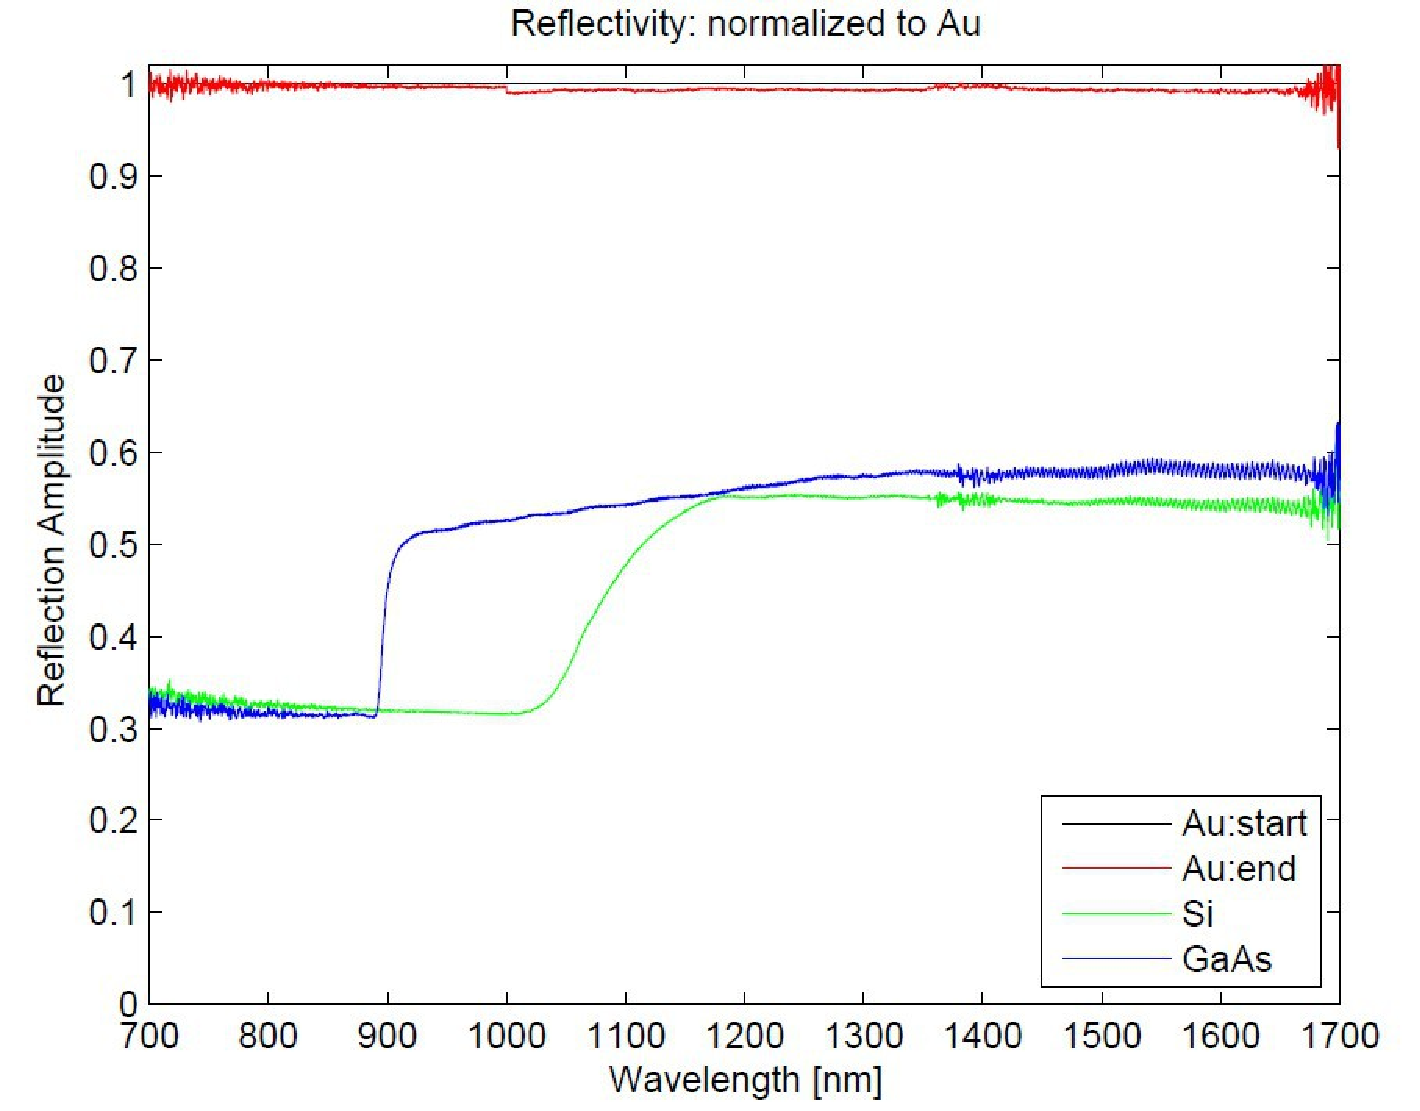
\includegraphics[width=\textwidth]{pictures/Data/reflecbulk}
  \label{reflecbulk}
\end{figure}

Figure~\ref{reflectCSNW} contrasts this with the measured absorption spectrum
of two types of GaAs core, AlGaAs shell nanowires (CSNWs): those grown on a
GaAs substrate (black), and the others heteroexpitaxially grown on a Si
substrate (red). The spectra show that both cases have the signature change of
reflectivity at badgap of GaAs, i.e., these are due to the GaAs/AlGaAs CSNWs,
not the substrate. Importantly, for the wavelength range of 700-1200nm these
core-shells which only occupy ~15\% of the volume compared to thin films of the
same height, reflect 2-4\% of light for the CSNWs grown on Si, and 3-7\% of
light for those grown on GaAs substrate. The beam-width of the incident light
being $\sim1{\mu}m$, this shows that only a few NWs are interrogated by ligth
and, normalized to volume, these wires absorb more than two orders of magnitude
more ligth than their thin-film counterparts.

\begin{figure}
  \caption{Reflectivity spectrum of GaAs/AlGaAs core-shells grown on Si (red) and GaAs (black) substrates shows, normalized to volume, nearly two orders of magnitude more absorption of ligth.}
  \centering
  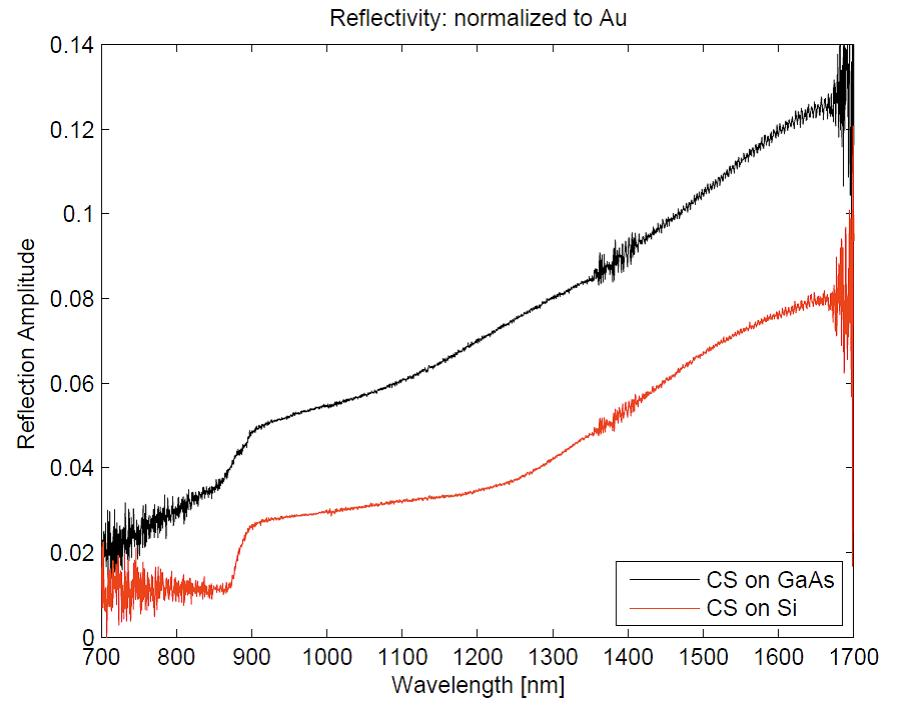
\includegraphics[width=\textwidth]{pictures/Data/reflectCSNW}
  \label{reflectCSNW}
\end{figure}

\section{Emission Enhancement} \label{Dust_data}

Figure~\ref{PL} compares room temperature micro photoluminescence (PL) spectrum
of bulk GaAs to CSNWs grown on GaAs, and two cuts of Si. The ratio of peak
luminescence of a) CSNWs on GaAs, B) CSNWs on Si[111] and c) Si(miscut)
substrates to bulk GaAs are, respectively, 923, 311 and 10. Considering the
beam width of $\sim1{\mu}m$, 5-10 NW were excited, yet emitted over three
order of magnitude more light compared to bulk.

\begin{figure}
  \caption{Photoluminescence of bulk GaAs, Core-Shell Nanowires grown on GaAs and Si.}
  \centering
  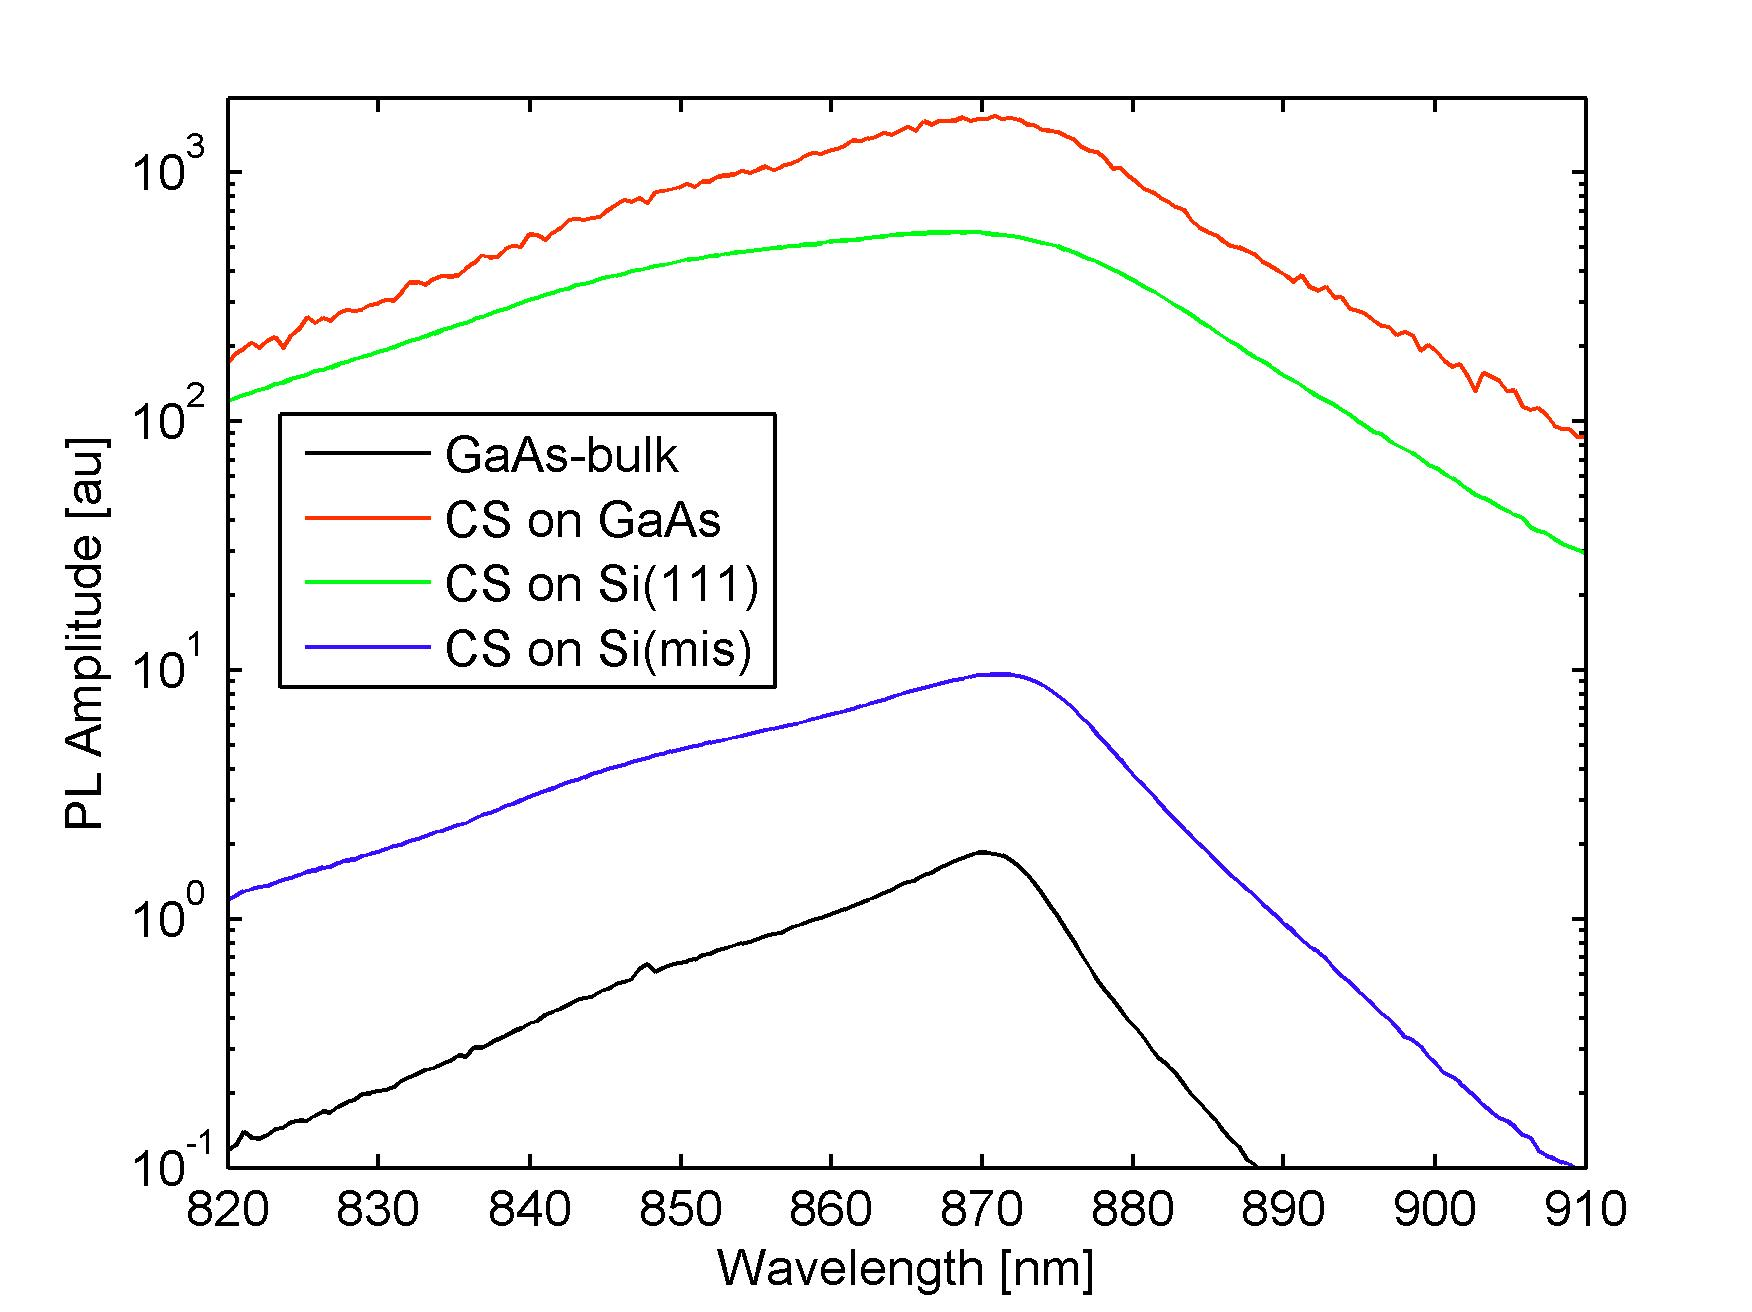
\includegraphics[width=\textwidth]{pictures/Data/PL}
  \label{PL}
\end{figure}

\section{Lasing} \label{data_lasing}

Photoluminescence (PL) of bulk GaAs to CSNWs grown on GaAs, and on two
directions of Si showed that normalized to the fraction of the volume that
these wires occupy, nearly 10,000 times more brightness is observed in these
wires compared to thin-film as in Fig.~\ref{PL}. In the case of stimulated
emission of light, the photon mode density $(1+u_\varepsilon)$ plays a crucial
role. Figure ~\ref{lasing} is the photoluminescence (PL) spectrum at various
optical pump intensities. As the excitation laser power increase beyond
$5{\mu}W$ a sudden and highly nonlinear increase in the emission intensity is
observed, with pronounced peaks emerging from 800nm to 850nm that rapidly grows
to become several orders of magnitude stronger than the background emission.
The lasing amplitude versus excitation power demonstrates a threshold of around
$5{\mu}W$, followed by saturation near $12{\mu}W$. This nonlinear threshold
behavior shows in detail in the L-L plot, (i.e., The pumping power intensity
(L) versus output light power intensity (L)) as in Fig.~\ref{expthreshold}. The
sharp peak has a full width half maximum (FWHM) that varies from 1.5 to 3.5 nm.
This remarkable behavior is achieved in the as-grown wires with no vertical
structure.

\begin{figure}
  \caption{Micro-Photoluminescence measurements with fs-pulsed, 532-nm laser excitation at 250kHz repetition rate shows lasing of the as-grown wires.}
  \centering
  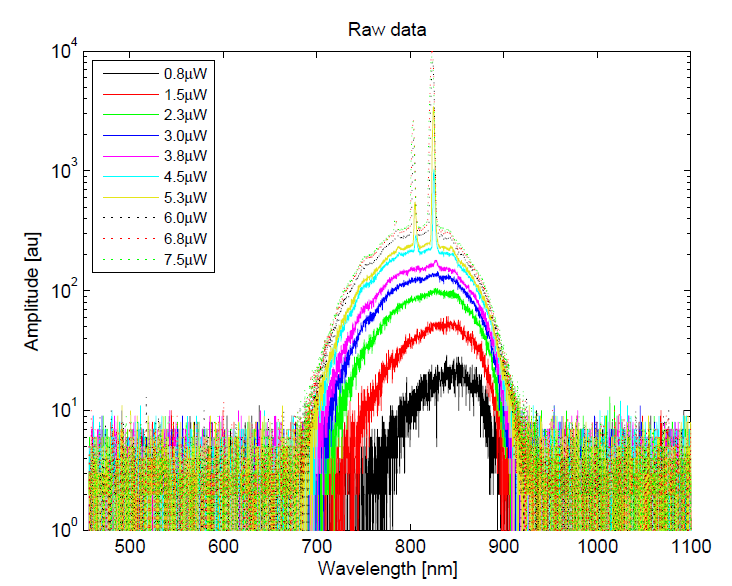
\includegraphics[width=\textwidth]{pictures/Data/lasing}
  \label{lasing}
\end{figure}

\begin{figure}
  \caption{\em{L-L curve of as-grown core-shell nanowire.} The pumping power intensity (L) versus output light power intensity (L) of as-grown core-shell nanowire operating at room temperature with a low threshold of $\sim10{\mu}W$ and followed by saturation near $22{\mu}W$.}
  \centering
  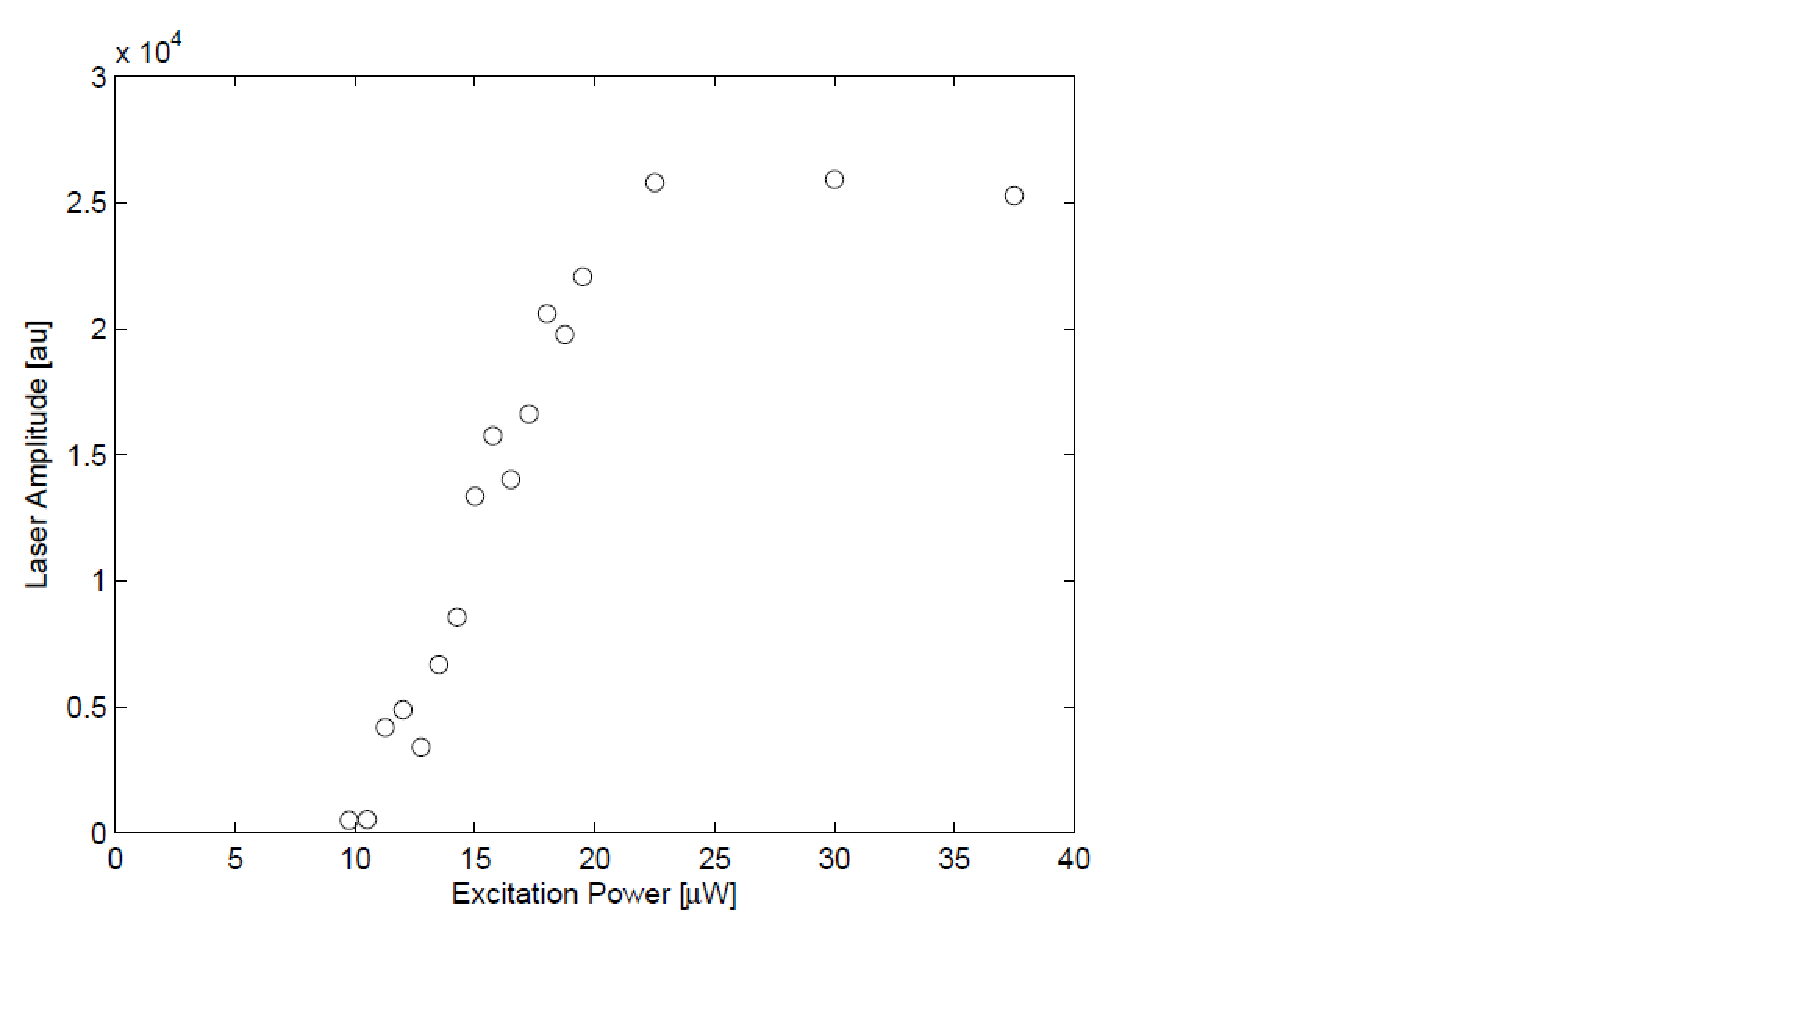
\includegraphics[width=\textwidth]{pictures/Data/expthreshold}
  \label{expthreshold}
\end{figure}
